\begin{frame}{Big Data Problem}
    \begin{itemize}
        \item Millions of matches played every day
        \item 40 of GB data generated per day in western europe alone
        \item New game versions requires a relearning of matches
    \end{itemize}
    Thus we have a big data problem. What is a Big Data?
\end{frame}

\begin{frame}{Big Data Definition}
    Usually defined by three factors:
    \begin{itemize}
        \item Volume
        \item Velocity
        \item Variety
    \end{itemize}
    LoL Data:
    \begin{itemize}
        \item Volume: 456GB static size
        \item Velocity: We wont consider
        \item Variety: Not a problem
    \end{itemize}
\end{frame}

\begin{frame}{Big Data Technology}
\centering 
\includegraphics[scale=0.4]{bigdataandcluster/hadoop.png}

\centering 
\includegraphics[scale=0.4]{bigdataandcluster/spark.png}
\end{frame}

\begin{frame}{Hadoop Distributed File System(HDFS)}
    \begin{itemize}
        \item Distributed file system 
        \item Hides complexity, seemlessly looks like a regular linux FS
        \item Master-worker achitecture
        \begin{itemize}
            \item Master(namenode) $\rightarrow$ file hiearchy, location of file blocks
            \item Worker(datanode) $\rightarrow$ stores the actual blocks locally
        \end{itemize}
    \end{itemize}
\end{frame}

\begin{frame}{Hadoop Distributed File System(HDFS)}
    \centering 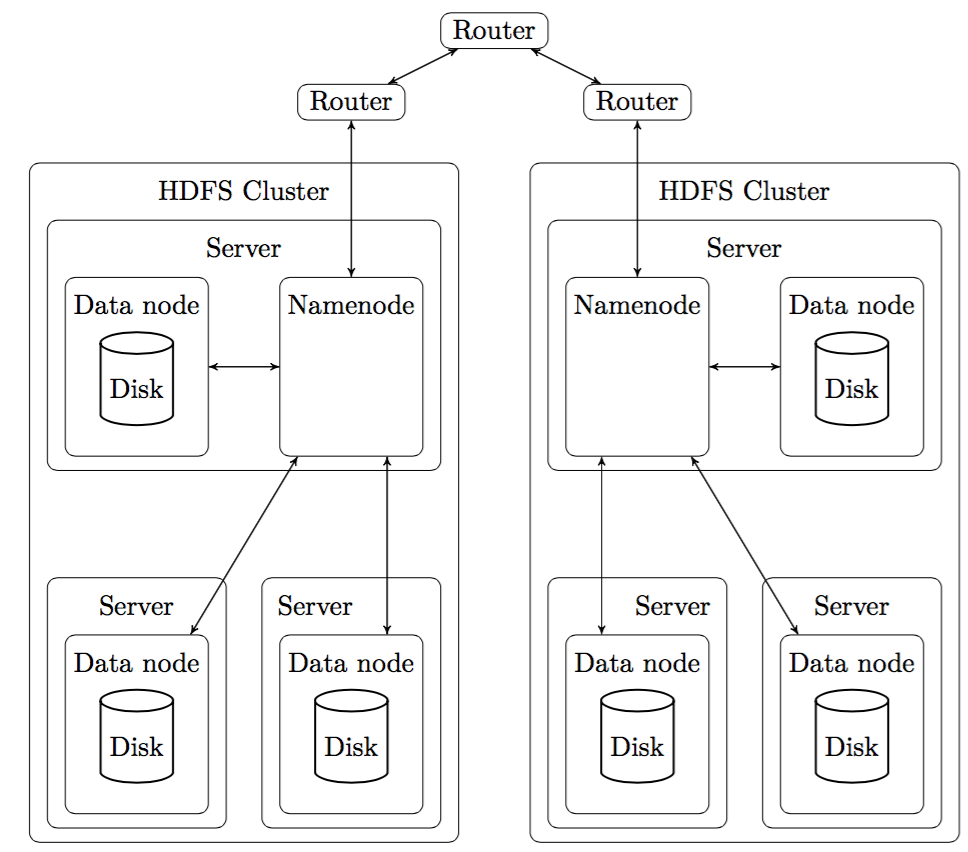
\includegraphics[scale=0.5]{bigdataandcluster/hdfs.png}
\end{frame}

\begin{frame}{MapReduce}
    \begin{itemize}
        \item Programming model for distributed computing
        \item Inspired by functional programmings \textbf{map} and \textbf{reduce} operations
        \begin{itemize}
            \item \textbf{Map} $(key1, value1) \rightarrow list<(key2, value2)>$
            \item \textbf{Reduce} $(key2, list<value2>) \rightarrow list<value2>$
        \end{itemize}
    \end{itemize}
    Example word count
    \begin{itemize}
        \item \textbf{Map} $(name, document) \rightarrow (word, 1)$
        \item \textbf{Reduce} $(word, list<1,\dots,1)>) \rightarrow list<(word,count)>$
    \end{itemize}
\end{frame}

\begin{frame}{Apache Spark}
    \begin{itemize}
        \item MapReduce implementation for distributed computing, compatible with hdfs
        \item Also master-worker architecture
        \item Excellent for iterative algorithms such as Logistic Regression
        \item High level programming environment
        \item Graphical UI for running programs
    \end{itemize}

\end{frame}
\begin{frame}{Apache Spark}
        \centering 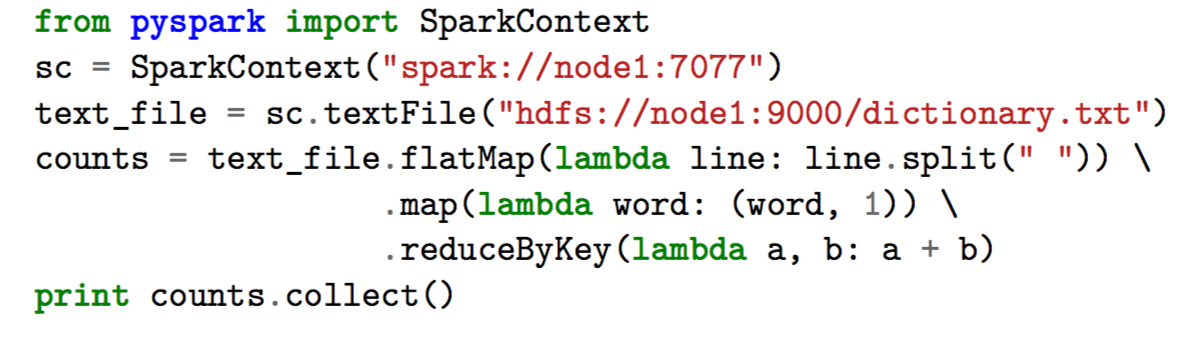
\includegraphics[scale=0.55]{bigdataandcluster/code.png}
\end{frame}


\begin{frame}{Cluster}
  \centering \includegraphics[width=0.8\textwidth]{bigdataandcluster/cluster2.jpg}
\end{frame}
\begin{frame}{Cluster}

    4 computers with hardware from $\thicksim$ 2008
      \begin{tabular}{|r|ccc|}
    \hline
      & CPU & Storage & Memory \\\hline
    1 & Dual core intel e8400 3Ghz & 220 GB 7200 RPM & 4GB DDR2 \\
    2 & Quad core intel q9400 2.66Ghz & 220 GB 7200 RPM & 8GB DDR2 \\\hline
  \end{tabular}
\end{frame}






